\documentclass[specialist,
               substylefile = spbu_report.rtx,
               subf,href,colorlinks=true, 12pt]{disser}

\usepackage[a4paper,
            mag=1000, includefoot,
            left=3cm, right=1.5cm, top=2cm, bottom=2cm, headsep=1cm, footskip=1cm]{geometry}
\usepackage[T2A]{fontenc}
\usepackage[utf8]{inputenc}
\usepackage[english,russian]{babel}
\ifpdf\usepackage{epstopdf}\fi

% Точка с запятой в качестве разделителя между номерами цитирований
%\setcitestyle{semicolon}


% Включать подсекции в оглавление
\setcounter{tocdepth}{2}

\graphicspath{{fig/}}

%----------------------------------------------------------------
\begin{document}

%
% Титульный лист на русском языке
%

% Название организации
\institution{%
    Санкт-Петербургский государственный университет \\
    Прикладная математика и информатика \\
    Прикладная кибернетика
}

\title{Научная иследовательская разбота}

% Тема
\topic{\normalfont\scshape%
Cравние на синтетических данных и на данных с Kaggle методов для рассчёта доверительных интервалов для 90, 99 квантилей}

% Автор
\author{Кривоносов Тимофей Игоревич}

% Научный руководитель
\sa       {М.\,В.~Юлдашев}
\sastatus {д.\,ф.-м.\,н., профессор}

% Рецензент
\rev      {П.\,П.~Петров}
\revstatus{к.\,ф.-м.\,н., доцент}

% Город и год
\city{Санкт-Петербург}
\date{\number\year}

\maketitle

\newpage
\tableofcontents
\newpage
\section{Введение}
В современном мире статистический анализ играет важную роль во многих областях, от науки до бизнеса. При работе с данными мы часто сталкиваемся с необходимостью оценки параметров и построения доверительных интервалов для различных квантилей распределений. Квантили представляют собой значения, разделяющие вероятностное распределение на равные части.

В данной курсовой работе мы сосредоточимся на сравнении методов для расчета доверительных интервалов для 90-го и 99-го квантилей на основе синтетических данных и данных, предоставленных платформой Kaggle. Синтетические данные являются созданными искусственным образом наборами данных, которые позволяют нам контролировать различные аспекты, такие как распределение, объем выборки и т.д. Данные, полученные с Kaggle, представляют собой реальные данные, предоставленные сообществом пользователей этой платформы.

Для синтезирования данных и проверки методов поиска доверительных интервалов для 90 и 99 квантилей в задаче сравнения производительности и задержки (latency), проведу следующие шаги:

\begin{itemize}
 
\item  Собрать данные: Запустите эксперименты или тесты, которые измеряют производительность и задержку вашей системы. Запишите результаты для каждого теста.

\item Подготовить выборки: Создайте выборки из результатов тестов, соответствующие каждому методу или условию, которое вы хотите сравнить. Например, если вы сравниваете два разных алгоритма, создайте две выборки, содержащие результаты для каждого алгоритма.

\item Анализировать выборки: Используйте статистические методы для анализа выборок и вычисления доверительных интервалов. Для нахождения доверительного интервала 90\% квантили, найдите 5-й и 95-й перцентили выборки. Для доверительного интервала 99\% квантили найдите 0.5-й и 99.5-й перцентили выборки.

\item  Проверьте методы поиска доверительных интервалов: Сравните результаты, полученные различными методами поиска доверительных интервалов. Убедитесь, что методы возвращают адекватные и интерпретируемые результаты.

\item Интерпретация результатов: Проанализируйте полученные доверительные интервалы и сделайте выводы относительно производительности и задержки системы. Например, если интервалы значительно отличаются для двух методов, это может указывать на значимые различия между ними.
\end{itemize}

Основной целью нашего исследования является провести сравнительный анализ методов расчета доверительных интервалов для выбранных квантилей на основе обоих типов данных. Это позволит нам оценить, насколько точно и надежно эти методы работают в различных условиях и с разными типами данных.

Ожидается, что результаты данного исследования помогут нам лучше понять применимость и эффективность различных методов для расчета доверительных интервалов на основе разных типов данных, что может быть полезным при принятии статистических решений в реальных ситуациях.
\newpage
\section{Методы нахождения доверительных интервалов}

Квантиль - это значение, которое разделяет упорядоченную выборку на две части таким образом, что заданный процент значений находится слева (ниже) этого значения, а оставшиеся значения находятся справа (выше). Например, 90-й квантиль (0.9-квантиль) разделяет выборку так, что 90\% значений находятся ниже этого значения.

Доверительный интервал для заданного квантиля позволяет оценить диапазон, в котором с определенной вероятностью находится истинное значение параметра. Например, доверительный интервал для 90-го квантиля указывает на диапазон значений, в котором с вероятностью 90\% будет находиться искомая величина.

\subsection{Наивный подход}

Наивный подход для поиска доверительного интервала для 90-го квантиля (или любого другого квантиля) является простым и интуитивным методом. Он основан на сортировке выборки значений и нахождении соответствующего элемента, который делит выборку на две части: одна содержит 90\% значений, меньших или равных этому элементу, а другая - 10\% значений, больших или равных ему.

Для нахождения доверительного интервала с использованием наивного подхода для 90-го квантиля, следуйте этим шагам:
    \begin{itemize}
        \item Упорядочите выборку значений в порядке возрастания (или убывания).
		\item Вычислите индекс элемента, который соответствует 90-му перцентилю, используя формулу: index = (90/100) * n, где n - размер выборки.
		\item Округлите индекс до ближайшего целого числа. Если индекс не является целым числом, возьмите следующее целое число больше него.
		\item Найдите значение, соответствующее округленному индексу в отсортированной выборке. Это будет значение, разделяющее выборку на 90\% и 10\% части.
		\item Доверительный интервал для 90-го квантиля будет состоять из значений, которые меньше или равны найденному значению.
    \end{itemize}
		
Например, если у вас есть выборка [1, 2, 3, 4, 5, 6, 7, 8, 9, 10] и вы хотите найти доверительный интервал для 90-го квантиля, вычисления будут следующими:
	\begin{itemize}	
        \item Сортировка выборки: [1, 2, 3, 4, 5, 6, 7, 8, 9, 10].
		\item Индекс = (90/100) * 10 = 9.
		\item Округленный индекс = 9.
		\item  Значение по округленному индексу: 9.
		\item Доверительный интервал: [1, 2, 3, 4, 5, 6, 7, 8, 9].
    \end{itemize}
        	
Наивный подход для поиска доверительных интервалов может быть простым и быстрым, но он не учитывает особенности распределения данных и может быть менее точным в некоторых случаях. Поэтому для более точных и надежных результатов рекомендуется использовать статистические методы, такие как методы максимального правдоподобия или бутстрэп.

\subsection{Бустерэп}

Метод бутстрэп — это статистический метод для оценки распределения параметров и построения доверительных интервалов. Он основан на идее повторного выбора с возвращением из исходной выборки.

Процедура бутстрэп состоит из следующих шагов:
\begin{itemize}
    \item Из исходной выборки размером n случайным образом выбираются наблюдения с возвращением, так что новая выборка также имеет размер n.
    \item На основе этой новой выборки вычисляется интересующая нас статистика (например, среднее значение или медиана).
    \item Шаги 1-2 повторяются множество раз (обычно от 1000 до 10 000), чтобы получить распределение статистики.
    \item C помощью полученного распределения статистики строятся доверительные интервалы.
\end{itemize}
Пример использования метода бутстрэп:
\newline
Предположим, у нас есть выборка размером 100 наблюдений и мы хотим построить доверительный интервал для среднего значения. Мы можем применить метод бутстрэп следующим образом:

\begin{itemize}
    \item Создаем множество бутстрэп-выборок путем случайного выбора 100 наблюдений из исходной выборки с возвращением.
    \item Для каждой бутстрэп-выборки вычисляем среднее значение.
    \item Полученные средние значения образуют распределение, которое отражает неопределенность вокруг истинного среднего значения.
    \item Используем полученное распределение для построения доверительного интервала, например, 95\% доверительного интервала будет содержать средние значения, лежащие между 2.5-м и 97.5-м процентилями этого распределения.
\end{itemize}

Таким образом, метод бутстрэп позволяет оценить статистическую неопределенность и построить доверительные интервалы для различных параметров на основе анализа повторных выборок из исходной выборки.

\subsection{Дельта подход}

Дельта метод является одним из способов нахождения доверительных интервалов для заданных квантилей. Он основан на аппроксимации нормальным распределением 
и использует центральную предельную теорему. Аппроксимация нормальным распределением - это метод приближения вероятностного распределения случайной величины нормальным (гауссовским) распределением. Он основан на центральной предельной теореме, которая утверждает, что сумма большого числа независимых и одинаково распределенных случайных величин имеет распределение, близкое к нормальному.

В дельта методе используется аппроксимация первого порядка (линейная аппроксимация) для построения доверительных интервалов. Он предполагает, что функция случайной величины может быть приближена линейной функцией ее математического ожидания и стандартного отклонения. Поэтому доверительный интервал строится, используя оценку математического ожидания и стандартного отклонения случайной величины, взятой с помощью производной этой функции. Дельта метод широко применяется при работе с нелинейными функциями случайных величин и позволяет получить аппроксимацию их доверительных интервалов.
\newline
Для нахождения доверительного интервала по дельта методу следуют следующие шаги:
\begin{itemize}
    \item Вычислить выборочное среднее ($\bar x$) и стандартное отклонение (s) на основе имеющейся выборки данных.
    \item Найти z-значение, соответствующее выбранному уровню доверия, часто это табличные значения (например, для уровня доверия 90\% это будет z = 1.645, а для 99\% - z = 2.576).
    \item Рассчитать половину ширины доверительного интервала ($\delta$), умножив z-значение на стандартное отклонение, деленное на квадратный корень из объема выборки: $\delta = z * (s / \sqrt n)$.
    \item На основе выборочного среднего и половины ширины интервала можно построить доверительный интервал: [$ \bar x - \delta$,$ \bar x  + \delta$].
\end{itemize}
Наглядный пример: 
\newline
Предположим, что у нас есть выборка из 100 наблюдений, и мы хотим построить 90\% доверительный интервал для среднего значения. После вычисления выборочного среднего ($\bar x$) и стандартного отклонения (s) находим z-значение для 90\% доверия, равное 1.645. Затем рассчитываем половину ширины интервала по формуле $\delta = 1.645 * (s / \sqrt 100)$. Итак, если $\bar x$ = 50 и s = 10, то $\delta = 1.645 * (10 / \sqrt 100) = 1.645$. Таким образом, получаем доверительный интервал [50 - 1.645, 50 + 1.645] = [48.355, 51.645].

Таким образом, дельта метод предоставляет нам инструмент для построения доверительных интервалов для заданных квантилей.
% \newline 
% Для расчета доверительного интервала для квантилей 90% и 99% методом дельты, вам понадобятся следующие шаги:

% Получите выборку данных, для которой вы хотите рассчитать доверительный интервал.
% Отсортируйте выборку по возрастанию.
% Рассчитайте индексы для квантилей, используя формулу: 
% index = (n - 1) * p
% , где 
% n
%  - размер выборки, а 
% p
%  - процентиль (например, 0.9 для 90\% или 0.99 для 99\%).
% Округлите полученные индексы вниз до ближайшего целого числа.
% Рассчитайте доверительные интервалы: 
% lower_bound = data[index]
%  и 
% upper_bound = data[index + 1]
% .
% Если индекс является целым числом, то 
% lower_bound
%  и 
% upper_bound
%  равны соответствующим значениям в выборке.
% Если индекс не является целым числом, то 
% lower_bound
%  и 
% upper_bound
%  будут линейно интерполироваться между двумя ближайшими значениями в выборке.
\newpage
\section{Cбор и генерация данных}

\subsection{Синтезированные данные}
    При создании тестовых данных для проверки методов поиска доверительного интервала следует учитывать следующие аспекты:
    \begin{itemize}
        \item    Известное распределение данных: 
        Выбрать распределение, которое соответствует данным или сценарию исследования. Например, нормальное распределение, равномерное распределение или экспоненциальное распределение.
        (В нашем случае необходимо проверить все)
        \item 	 Размер выборки: 
        Определить размер выборки, который будет использоваться для генерации данных. (1000 эл)
        \item 	 Генерация случайных чисел:
        Использовать подходящий генератор случайных чисел, чтобы создать данные, соответствующие выбранному распределению и параметрам. 
        \item 	 Повторяемость
        Убедится, что тестовые данные повторяемы, то есть при каждом запуске теста они будут генерироваться с одинаковыми значениями.
    \end{itemize}  
     
    Во время создания программы для генерации данных необходимо учесть, что у каждого метода есть хорошие стороны и обратные, поэтому при синтезе нужно подготовить выборки как одного вида, так и другого. Для этого будем использовать разные распределения: нормальное, равномерное и экспоненциальное. После проверим каждый из методов и проведем анализ.
    Программа для создания выборок находится в приложении 1 или на \href{https://github.com/krivonosovti/QuantileCIComparison/blob/main/DataFactory.py}{GitHub}.
    
\subsection{Данные из Kaggle}
    Также следует проверить методы на данных созданных сообществом программистов и аналитков. Для этого зарегестрируемся на рессурсе \href{https://www.kaggle.com}{Kaggle} (Kaggle - это платформа для соревнований по анализу данных и машинному обучению. Она предоставляет сообществу специалистов по данным доступ к наборам данных, инструменты для исследования и моделирования данных, а также возможность участвовать в соревнованиях, где участники решают реальные проблемы с использованием машинного обучения и статистического анализа. Kaggle также предлагает образовательные материалы, форумы и средства для сотрудничества над проектами.)



\newpage
\section{Анализ и сравнение разобранных методов}
    \subsection{Применение методов}
        Создадим три программы, каждая из которых на вход получает файл с выборками, находит доверительный интервал, время выболнения метода и False Positive Rate. Выходными данными я вляется фал ".txt" имеющий вид
       \newline
      \textit{sample1 90 или 99 доверительный интервал [-1.599138 ; 1.65090] Время поиска 90 интервала  6.91413879395 FPR 0.098}
        Программы и выходные данные находятся в Приложении 2 или на GitHub.
    \subsection{Анализ и сравнение методов}
    Получив результаты от каждого метода сравним их (программа - Приложение 3).
    Самым быстрым методом я вляется (...) со средней скоростью:
    В свою очередь самым 
    \subsection{Подведение итогов}

\newpage
\section {Заключение}
more...
\newpage
\section {Приложение}
\begin{enumerate} 
    \item Программа генерации выборок:
    \newline
    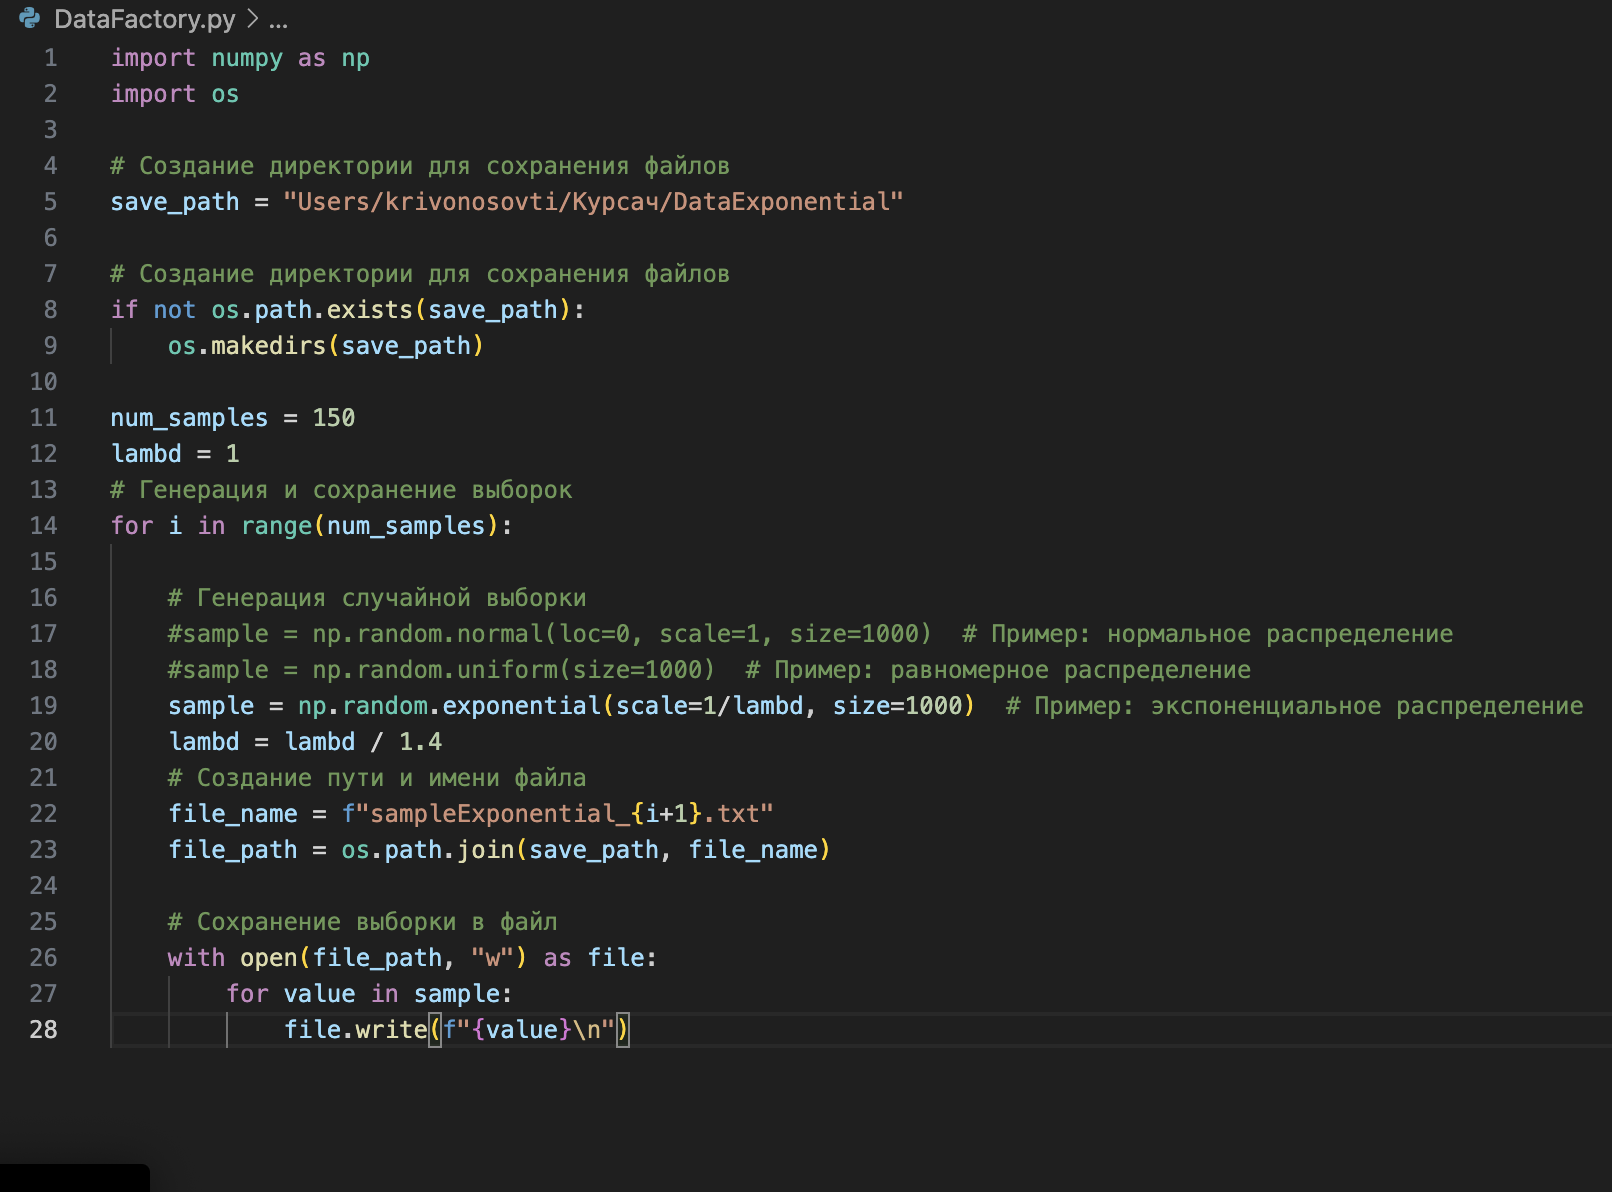
\includegraphics[width = 6in]{image1.png}


\end{enumerate} 
        
\end{document}